\begin{activity}{Thermal Refraction by Insulating Sediments}

\section*{Purpose}
To build intuition for how low-conductivity surface layers redistribute
temperature gradients without changing the total heat flow.

{\color{red}
\section*{Learning Outcomes}

By the end of this activity, you should be able to:
\begin{itemize}
  \item Apply Fourier's law to explain why the temperature gradient is steeper in low-conductivity material at constant heat flow.
  \item Sketch temperature--depth profiles for a layered crust and identify where isotherms are compressed or stretched.
  \item Predict which crustal section reaches higher interface temperatures and explain why.
  \item Discuss the implications of sedimentary basins for geothermal gradient measurements and geothermal energy potential.
\end{itemize}
}

\section*{Geological Context}
Consider two continental regions with identical basal heat flow from the mantle:
\begin{itemize}
  \item Region A: crystalline crust exposed at the surface.
  \item Region B: crystalline crust overlain by a thick sedimentary basin.
\end{itemize}
\begin{figure}
  \centering
  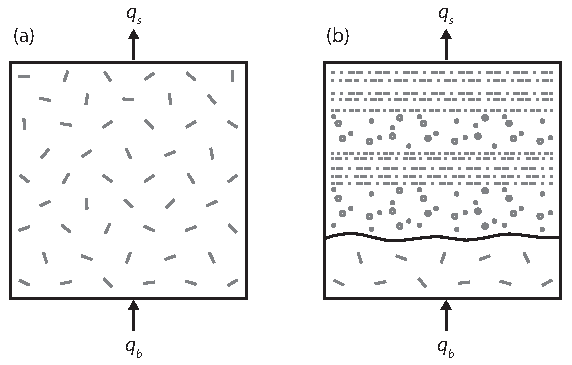
\includegraphics[]{figures/ig_vs_sed.pdf}
  \caption{Two continental terranes: (a) igneous crust, (b) sedimentary basin over igneous crust.}
  \label{fig:ivs}
\end{figure}

The sediments are dominated by shales and porous clastic rocks with lower
thermal conductivity than basement rock.

\section*{Assumptions}
\begin{itemize}
  \item Steady-state heat flow.
  \item No internal heat production in sediments.
  \item Heat flow is vertical and laterally uniform.
\end{itemize}

\section*{Tasks}
\begin{enumerate}
  \item Using Fourier's law,
  \[
    q = -k \frac{dT}{dz},
  \]
  explain qualitatively how the temperature gradient differs between
  sediments and basement.
  \answerbox[3cm]

  \item Sketch temperature versus depth for both regions on the same axes.
  Clearly label:
  \begin{itemize}
    \item sediment thickness,
    \item basement,
    \item relative steepness of gradients.
  \end{itemize}
  \answerbox[6cm]

  \item Indicate where isotherms are compressed and where they are stretched.
  \answerbox[3cm]

  \item Which region would exhibit a higher temperature at the sediment--basement
  interface? Explain why.
  \answerbox[3cm]
\end{enumerate}

\section*{Discussion}
\begin{itemize}
  \item How does the presence of sediments affect measured geothermal gradients?
  \answerbox[2cm]
  \item Which region would you expect to have higher geothermal potential?
  \answerbox[2cm]
  \item Why might sedimentary basins be favorable geothermal targets?
  \answerbox[2cm]
\end{itemize}

{\color{red}
\section*{Key Ideas}

{\color{blue}
\textbf{Heat flow is conserved; temperature gradient is not.} At steady state in a laterally uniform column without heat production, the heat flow $q$ is constant with depth. Because $q = -k\,dT/dz$, a low-conductivity layer must have a steeper gradient to carry the same heat flux. This is thermal refraction.

\begin{figure}[h]
\centering
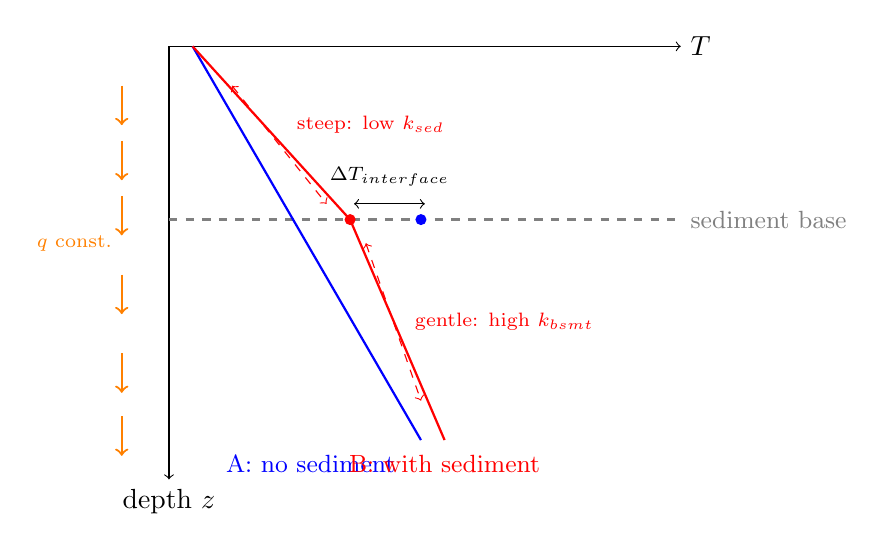
\begin{tikzpicture}[scale=1.0]
  % Axes
  \draw[->] (0, 0) -- (6.5, 0) node[right] {$T$};
  \draw[->] (0, 0) -- (0,-5.5) node[below] {depth $z$};

  % Layer boundary
  \draw[dashed, gray, thick] (0,-2.2) -- (6.5,-2.2);
  \node[right, font=\small, gray] at (6.5,-2.2) {sediment base};

  % Region A (no sediment): single gradient through basement
  \draw[thick, blue] (0.3, 0) -- (3.2,-5.0);
  \node[blue, font=\small] at (1.8, -5.3) {A: no sediment};

  % Region B (with sediment): steep in sediment, gentle in basement
  \draw[thick, red] (0.3, 0) -- (2.3,-2.2);   % steep in sediment
  \draw[thick, red] (2.3,-2.2) -- (3.5,-5.0); % gentle in basement
  \node[red, font=\small] at (3.5, -5.3) {B: with sediment};

  % Slope annotations
  \draw[<->, red, dashed] (0.8, -0.5) -- (2.0,-2.0);
  \node[red, font=\scriptsize, right] at (1.5,-1.0) {steep: low $k_\text{sed}$};
  \draw[<->, red, dashed] (2.5,-2.5) -- (3.2,-4.5);
  \node[red, font=\scriptsize, right] at (3.0,-3.5) {gentle: high $k_\text{bsmt}$};

  % Heat flow arrows (constant q)
  \foreach \y in {-0.5,-1.2,-1.9,-2.9,-3.9,-4.7} {
    \draw[->, orange, thick] (-0.6,\y) -- (-0.6,\y-0.5);
  }
  \node[orange, font=\scriptsize, left] at (-0.6,-2.5) {$q$ const.};

  % Interface temperature labels
  \fill[blue]  (3.2,-2.2) circle (2pt);
  \fill[red]   (2.3,-2.2) circle (2pt);
  \draw[<->] (3.25,-2.0) -- (2.35,-2.0);
  \node[font=\scriptsize, above] at (2.8,-1.9) {$\Delta T_\text{interface}$};
\end{tikzpicture}
\caption{Thermal refraction: constant heat flow (orange arrows) produces a steeper gradient in low-conductivity sediments (red, Region B) than in basement (blue, Region A). The sediment--basement interface in Region B is hotter than the equivalent depth in Region A.}
\end{figure}
}

\textbf{Low-conductivity sediments act as thermal insulators.} Isotherms are compressed (elevated) within and beneath low-conductivity sediments. The same basal heat flow produces higher temperatures at the sediment--basement interface when a sedimentary layer is present.

\textbf{Geothermal gradients measured in sedimentary basins need correction.} A borehole geothermal gradient measured in shale does not represent the gradient in the underlying crystalline basement. Applying Fourier's law to correct for conductivity contrasts is essential before comparing heat flow across different lithological settings.
}

\end{activity}
